\subsection{Regios}
\label{sec:regios}

\begin{center}
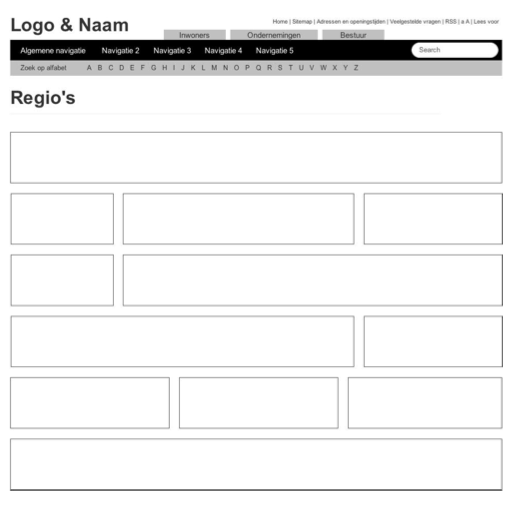
\includegraphics[scale=.5]{img/regions.png}
\end{center}

Op de pagina zijn de volgende regio's gedefinieerd. Aan de boven- en onderkant van de pagina zijn regio's over de hele breedte van de pagina beschikbaar. Daarnaast kent de template de volgende opstellingen.

\begin{description}
\item[Drie kolommen - smal / breed / smal] Deze opzet bestaat uit drie regio's waarbij de linker en rechter smaller zijn dan de middelste regio.
\item[Twee kolommen - smal / breed] Deze opzet bestaat uit twee regio's waarbij de linker regio smaller is dan de rechter.
\item[Twee kolommen - breed / smal] Deze opzet bestaat uit twee regio's waarbij de linker regio breder is dan de rechter.
\item[Drie kolommen] Deze opzet bestaat uit drie regio's die allen even breed zijn.
\end{description}